\section{Off Product Inspector Tooling}

  The Off Product Inspector (OPI) was made so that people in editorial and partner marketing and non technical team members, could view the data that
  should be available to partners at that moment. It allows users to search for pids (unique identifiers) and titles of brands, series and episodes
  and then view the data of these items. I worked on two main things to extend this project, upgrade to support our new v2 catalogues and add the 
  Deeplink Generator.

  \subsection{Support v2 Catalogues}
  The OPI originally was designed to support the v1.1 catalogue, however the catalogue had been extended to v2 which included different data and also 
  had 3 \textit{horizon catalogues}.
  \begin{itemize}
    \item \textbf{v2.0 catalogue} - Contains all data, both what is currently available and unavailable on iPlayer.
    \item \textbf{v2.0 0-day catalogue} - Contains data that is on iPlayer right now.
    \item \textbf{v2.0 8-day catalogue} - Contains data that is on iPlayer right now and also contains things that will be available within 8 days.
  \end{itemize}

  Partners are being encouraged to move over to the new v2 version of the catalogue so its good to be able to see what theses catalogue should offer.
  Me and a fellow junior software engineer began by working on the \textit{spike} for the project. A spike is a task thats aim is to gain knowledge
  \todo[noline, size=\small]{B5, P3}
  and information on ahead of doing the work. This can often times mean creating a small MVP to show that it is possible. I talk about this and other
  software lifecycle issues in the \textbf{Software Engineering-1.pdf} document. The spike we created was an MVP that allowed the switching between 
  catalogue, however the code was not refined, there was no tests written and zero documentation, this would all come later. We then showed what we 
  had come up with to the team and then began the process of breaking the work down into slices/tickets.

  \vspace{0.2cm}

  I had never done or heard of a \textit{spike} before doing this for the OPI. It's easy to get carried away and go beyond the scope of the spike.
  Towards the end of this spike I began writing some tests for certain things but learned that this was not part of what a spike was. When doing 
  another spike for the schedules ingester, I took this lesson and stayed within the scope. This was also the first time I had been given a task that
  was UI based. \todo[noline, size=\small]{L2, L3, L7}
  This is an area I have much more knowledge in from my own teachings and allowed me to help/teach my colleague I was spiking with learn
  about how things like React hooks work and the interplay between React and Next.js.
  Further along in the project I also suggested that we move to a newer way of writing css and components called \textit{styled components}. Some benefits of
  these are:
  \todo[noline, size=\small]{T2}
  \begin{itemize}
    \item Styles are not separate from the component itself, making it easier to debug.
    \item Styled components can take props to easily customise aspects of a components style.
    \item Default html tags are given a more meaningful name, making it easier to understand the role of a tag.
  \end{itemize}

  Below is an example of the difference between using styled components and styling using SaSS (Syntactically Awesome Style Sheets).

  \begin{figure}[H]
    \centering
    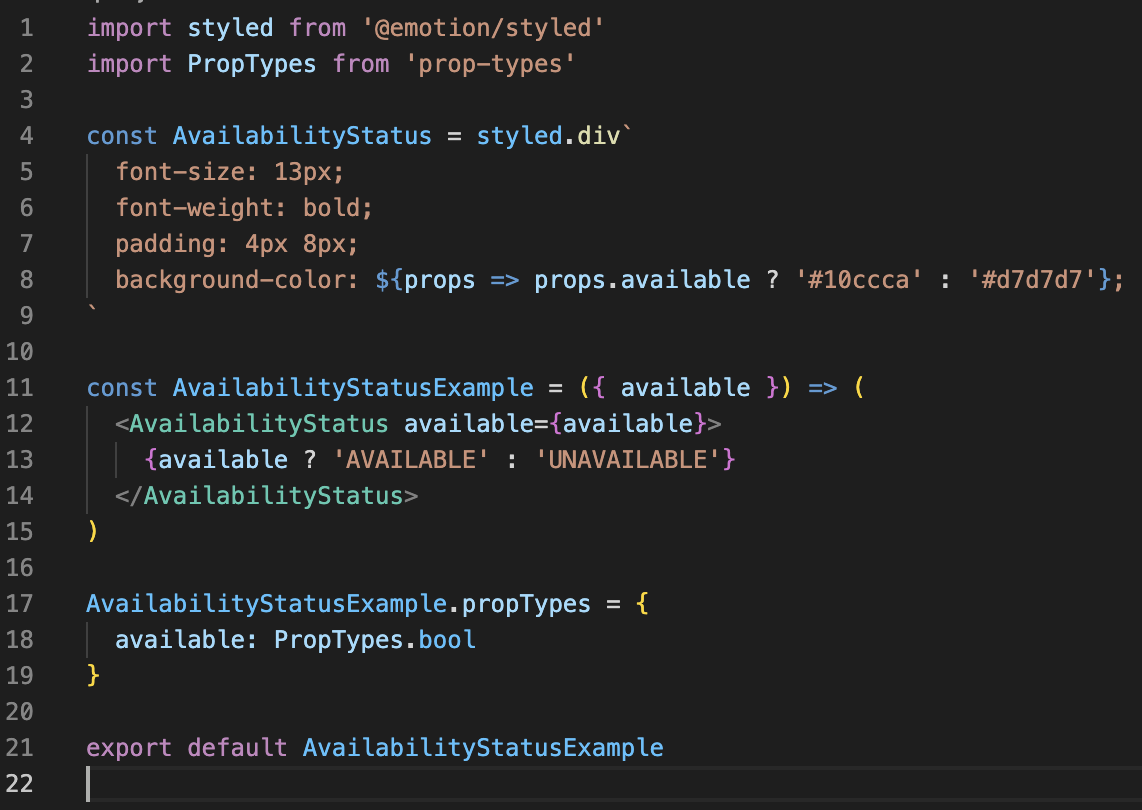
\includegraphics[width=6cm, height=4cm]{assets/StyledCompsOldJSX.png}
    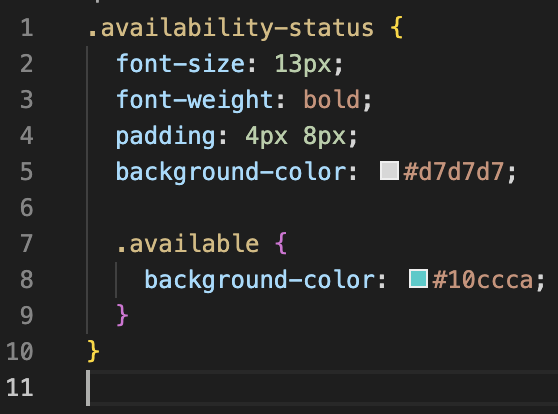
\includegraphics[width=6cm, height=4cm]{assets/styledCompsOldCSS.png}
    \caption{Screenshots of how not using styled components would work, JSX on left, SCSS on right.}
    \label{fig:oldStyling}
  \end{figure}

  \begin{figure}[H]
    \centering
    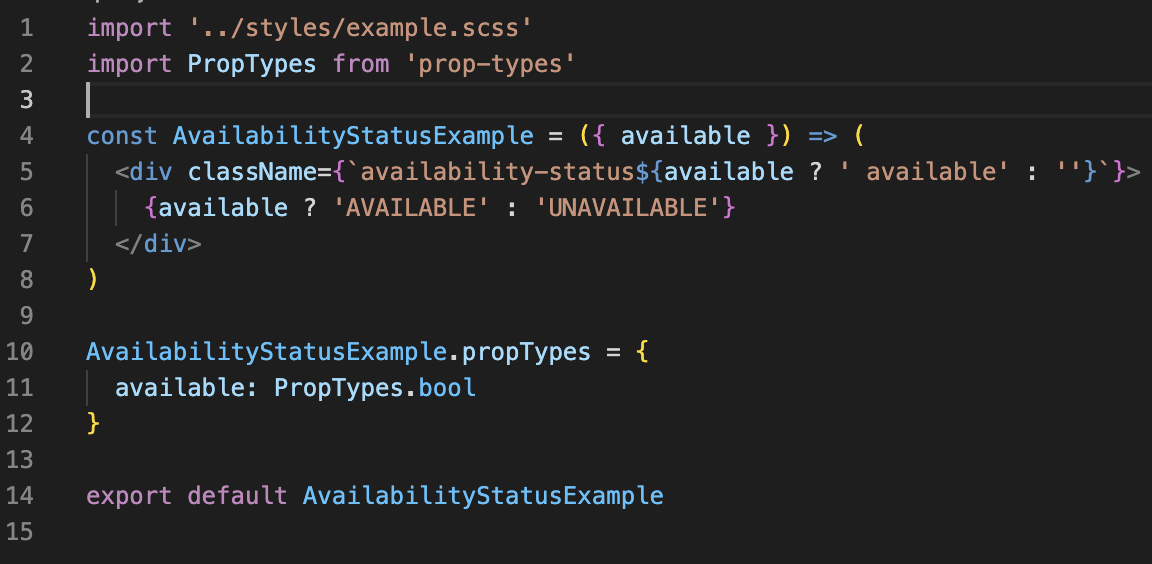
\includegraphics[width=8cm]{assets/styledCompsNew.png}
    \caption{Screenshot of how it looks using styled components.}
    \label{fig:newStyling}
  \end{figure}

  \subsection{Deeplink Generator}
  Deeplink generator stuff here.

    \subsubsection{Deeplink Generator Presentation}
    \todo[noline, size=\small]{P2, P3}
    On the 18th of July 2023 I presented at the Partnerships show n' tell meeting on behalf of my team. I presented the work we did for the
    deeplink generator and have included the slides in a separate document.

    This was the first time I've presented anything to a larger group of people and I was nervous going in. The presentation was short, due to the work
    being discussed not being very large, however it still took around 5 -7 minutes for the whole presentation. Overall I'm happy with how I managed the 
    presentation and with the presentation itself. It's something I should do more of in the future to become more comfortable with these kinds of things.
    For future I would take my time more when going through the slides. I felt like I rushed a little bit due to my nerves, however I feel like this is 
    something that comes with practice and being the the situation. 

  \subsection{Personal feedback on OPI}
  \todo[noline, size=\small]{P2, P3, L9, L10}
  I show the questions and feedback I received in the document \textbf{Feedback Form Output.docx}. I also go into a discussion of this in the document
  \textbf{Leaderships-1.pdf}.

  Reflecting now (August 2023) on the goals at the end of that assignment:
  \begin{itemize}
    \item \textbf{Pass AWS practitioner foundational} - I think I've outgrown this aim naturally. My skills and understanding of AWS is much greater than
    that of which I'd be assessed on. I am deffinately still interested in gaining some qualifications in AWS, however I would prefer for now to focus on 
    finishing my masters/apprenticeship rather than do that. In the future I will look into doing the develop or solutions architect certifications.
    \item \textbf{Improve input in meetings} - This is something I've got better at, partly due to me learning more about what we do as a team and therefore
    feeling less \textit{'imposter syndrome'} when giving out ideas.
    \item \textbf{Attend BBC mentoring training} - I am currently on the wait-list for this course.
  \end{itemize}

\newpage